
\documentclass{article}
\usepackage[utf8]{inputenc}
\usepackage{amsmath}
\usepackage{graphicx}
\usepackage{hyperref}
%\documentclass{article}
\usepackage{hyperref}


\sloppy

\title{Simulation of Ideal Gas Dynamics and Verification of Maxwell-Boltzmann Distribution}
\author{Federico Mastroforti}
\date{\today}

\begin{document}

\maketitle
\begin{abstract}
    This paper focuses on the simulation of an ideal gas using Python code. It explores the verification of the Maxwell-Boltzmann distribution of velocities, studies the mixing of two gases, and examines the impact of specific gas collision settings. The results are validated through simulations and theoretical analysis.
\end{abstract}

\tableofcontents

\section{Introduction}
The study of gas dynamics is fundamental in understanding various physical phenomena. This paper presents a simulation of an ideal gas using Python, with a focus on verifying the Maxwell-Boltzmann distribution of velocities. The investigation extends to the mixing of two gases and explores the impact of different collision settings.

\section{Simulation of an Ideal Gas}
\subsection{Maxwell-Boltzmann Distribution}
The Maxwell-Boltzmann distribution describes the statistical distribution of velocities in an ideal gas. In this study, we simulate the behavior of an ideal monoatomic gas in two dimensions, where each particle has only two translational degrees of freedom. Unlike the three-dimensional model originally developed by Boltzmann, our focus is on the two-dimensional case.

To accurately model this system, we need to derive the correct probability density function (PDF) for the velocity magnitude. While the classic Maxwell-Boltzmann distribution applies to three dimensions, the distribution of the speed in two dimensions does not follow the same pattern. Instead, it adheres to the Rayleigh distribution.

In our simulation, we first validate that the velocity distribution of the gas particles matches the Rayleigh distribution, which is the appropriate distribution for the magnitude of velocities in a two-dimensional ideal gas. By comparing the simulated data with the theoretical Rayleigh distribution, we confirm that our model accurately represents the behavior of a two-dimensional ideal gas.

Let’s derive the Rayleigh distribution for the magnitude of velocity. Consider the relationship between the components of the velocity and its magnitude:

\[
v_x^2 + v_y^2 = v^2,
\]

where \( v_x \) and \( v_y \) are the components of the velocity in the \( x \) and \( y \) directions, respectively, and \( v \) is the magnitude of the velocity.

It is known that the probability density functions (PDFs) of the velocity components \( v_x \) and \( v_y \) follow a Gaussian distribution with mean 0 and standard deviation \( \sigma \), where:

\[
f_{v_x}(v_x) = \frac{1}{\sqrt{2 \pi \sigma^2}} \exp \left( -\frac{v_x^2}{2 \sigma^2} \right),
\]

\[
f_{v_y}(v_y) = \frac{1}{\sqrt{2 \pi \sigma^2}} \exp \left( -\frac{v_y^2}{2 \sigma^2} \right),
\]

and where \( \sigma \) is given by:

\[
\sigma = \sqrt{\frac{k_B T}{m}},
\]

This Gaussian behavior of the velocity components arises from the Central Limit Theorem, as the velocity of a particle is the result of numerous small random changes due to a high number of interactions between particles. This theorem ensures that the sum of many independent random variables, each with a finite mean and variance, will tend to be normally distributed.

To find the PDF of the magnitude of velocity \( v \), we use the fact that \( v_x \) and \( v_y \) are independent Gaussian variables. The joint probability density function (PDF) of \( v_x \) and \( v_y \) is given by:

\[
f_{v_x, v_y}(v_x, v_y) = f_{v_x}(v_x) \cdot f_{v_y}(v_y) = \frac{1}{2 \pi \sigma^2} \exp \left( -\frac{v_x^2 + v_y^2}{2 \sigma^2} \right)
\]

To find the probability of finding a particle with velocity components within the ranges \( v_x \) to \( v_x + dv_x \) and \( v_y \) to \( v_y + dv_y \), we have:

\[
P(v_x \leq V_x < v_x + dv_x, \; v_y \leq V_y < v_y + dv_y) = f_{v_x, v_y}(v_x, v_y) \cdot dv_x \cdot dv_y
\]

To get the probability of finding a particle with velocity magnitude within the range \( v \) to \( v + dv \), we multiply the joint distribution by the infinitesimal surface \( 2 \pi v \, dv \) defined on the plane of velocities:

\[
P(v \leq V < v + dv) = \int_{v_x^2 + v_y^2 \in [v^2, v^2 + 2v \, dv]} f_{v_x, v_y}(v_x, v_y) \, dv_x \, dv_y
\]

The infinitesimal area on the plane of velocities is:

\[
\text{Area} = 2 \pi v \, dv
\]

Thus, the PDF of the magnitude \( v \) is:

\[
f_v(v) = \frac{f_{v_x, v_y}(v_x, v_y)}{2 \pi v} \text{Area}
\]

Substituting the joint PDF:

\[
f_v(v) = \frac{1}{2 \pi \sigma^2} \exp \left( -\frac{v^2}{2 \sigma^2} \right) \cdot \frac{1}{2 \pi v} \cdot 2 \pi v
\]

Simplifying:

\[
f_v(v) = \frac{v}{\sigma^2} \exp \left( -\frac{v^2}{2 \sigma^2} \right)
\]

This is the Rayleigh distribution for the magnitude of the velocity.

\section{Python Implementation and File Descriptions}
The simulation is implemented in Python and organized into multiple files for clarity. Below is a brief overview of each component:
\subsection{particle.py}
This file defines the \texttt{Particle} class, which encapsulates key parameters of the simulation such as position and velocity. It also includes attributes for coloring the particle based on its current velocity and stores the history of position, velocity, and velocity magnitude. This historical data is crucial for calculating the total energy of the system and for animating the simulation over time.

\subsection{physics\_engine.py}
This file contains the \texttt{PhysicsEngine} class, responsible for managing the time evolution of the system. It implements functions to handle collisions with walls (using simple reflections) and collisions between particles (for which a more detailed explanation of the velocity update method will be provided later). It also manages the time step of integration, the total number of steps, and the update of particle colors.

\subsection{initial\_state.py}
This file defines several methods for setting initial conditions. The \texttt{test\_initial} method is used for testing purposes, while \texttt{initial\_random\_state} initializes particles with positions uniformly distributed within the box (ensuring no overlap with other particles or walls) and velocity components that are also uniformly distributed. The \texttt{initial\_trigger} method sets most particles almost stationary, with one particle (the ``trigger'') launched at high speed. This setup allows us to observe the distribution of the gas particles as it evolves to a Maxwell-Boltzmann distribution.

\subsection{main.py}
This file sets up the simulation framework, initializes necessary parameters, and contains the code for displaying the simulation. For each time step, a frame showing the system's state and a histogram of velocity magnitudes, overlaid with the theoretical Maxwell-Boltzmann curve, is saved in a folder named \texttt{frames}. After the simulation completes, a video of the simulation is created using the following command:

\begin{verbatim}
ffmpeg -r 24 -i frames/frame_%04d.png -vcodec libx264 -pix_fmt yuv420p simulation.mp4
\end{verbatim}

This command generates a video named \texttt{simulation.mp4} from the sequentially saved frames.

% \subsection{Code}
% We will rpovide some more code later. Especially the output velocity after a collition and in Appendix the clarification keeping in mind that equal module velocities in input doesnt necessary result in output velocities nom equal.
\subsection{Results}
As time progresses, the velocity distribution converges to the Maxwell-Boltzmann distribution, regardless of the initial state of the system and the initial distribution of velocities. This convergence occurs independently of the initial conditions, demonstrating that the system naturally evolves towards the Maxwell-Boltzmann distribution as expected.

% Add a figure with a caption
\begin{figure}[h] % 'h' places the figure approximately here
    \centering
    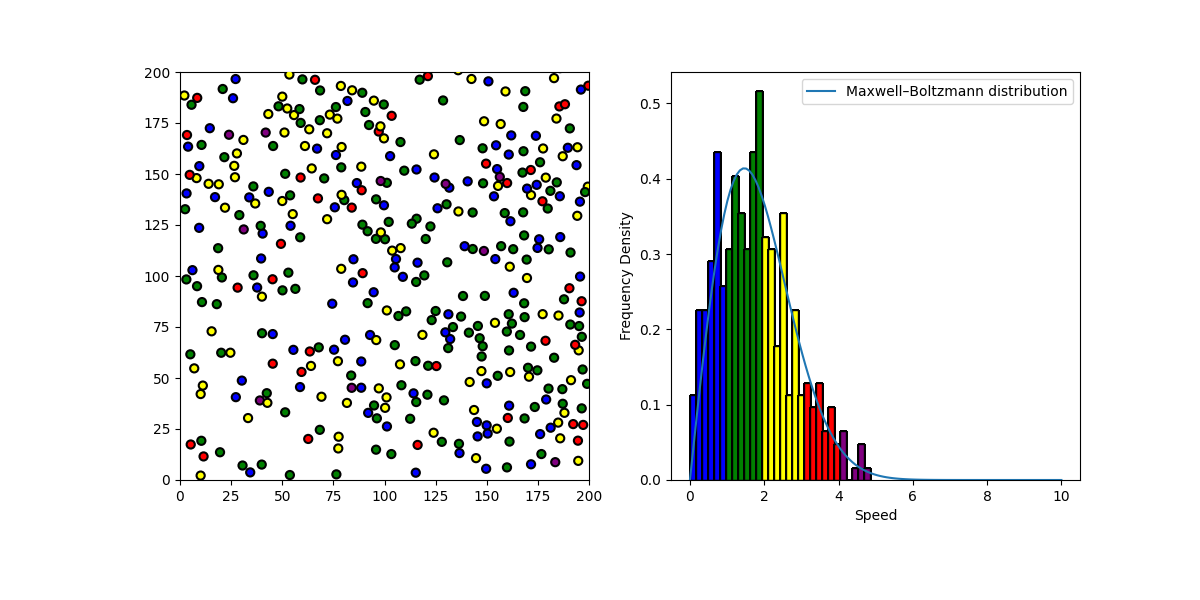
\includegraphics[width=0.8\textwidth]{Sing_gas_MB.png} % Replace with your image file name
    \caption{Distribution of velocities after thermalization. The figure shows how the velocity distribution (coloured) approaches the Maxwell-Boltzmann distribution (in blue).}
    \label{fig:velocity_distribution} % Label for referencing the figure
\end{figure}

\section{Mixing of Two Gases}
\subsection{Simulation of Gas Mixing}
We extend our simulation to study the mixing of two gases. The properties of each gas, as well as the mixing process, are analyzed in detail. The code for simulating the two gases allows for flexibility in choosing the size and mass of the particles, along with their initial velocity distribution, which determines their energy and temperature. At the start of the simulation, the two gases are separated, each occupying one half of the box. As the simulation progresses, the gases begin to mix.

As expected, the total energy of the system remains constant throughout the process, as does the average energy per particle. Although the energies of the individual gases change during mixing, their combined energy remains constant. Through testing, we verified that as time passes, the two gases tend to reach an equilibrium temperature.

In this case, we are not only interested in studying the velocity distributions of each gas separately, but we also aim to analyze the distribution of the velocity magnitudes by considering the two mixing gases as a single, combined system.

We derived the theoretical distribution for the combined system and verified it through our simulations, confirming that the behavior aligns with theoretical expectations.

\subsection{Combined System Velocity Distribution}
We aim to derive the Maxwell-Boltzmann distribution for the combined system of two gases. Each gas follows its own Rayleigh distribution (a form of the Maxwell-Boltzmann distribution) with unique temperatures (that will change through time due to thermalizaion) and masses, and therefore distinct values of \( \sigma \).

Our goal is to find the probability density function (PDF) of the velocity magnitude \( v \) for the combined system. We start by determining the probability that, for any random particle in the gas, its velocity falls between \( v \) and \( v + dv \), which can be expressed as:

\[
P(v \leq V < v + dv) = f_{\text{combined}}(v) \cdot dv
\]
Applying Bayes' theorem we get: 
\[
    P(v \leq V < v + dv) = P(v \leq V < v + dv | 1)*P_1 + P(v \leq V < v + dv | 2)*P_2
\]

Where \(P(v \leq V < v + dv | 1)\) and \(P(v \leq V < v + dv | 2)\) are the probabilities of finding a particle with velocity falling between \( v \) and \( v + dv \) given it belongs respectively to the first or second gas; they can be simply expressed as:

\[
P(v \leq V < v + dv|i) = f_{\text{i-gas}}(v) \cdot dv 
\]

and \(f_{\text{i-gas}}(v)\) is the PDF of the i-th gas.

The weights \( P_1 \) and \( P_2 \) are the probabilities of selecting a particle from the first and second gas, given by:

\[
P_1 = \frac{N_1}{N_{\text{total}}}, \quad P_2 = \frac{N_2}{N_{\text{total}}}
\]

Here, \( N_1 \) and \( N_2 \) represent the number of particles in the first and second gases, and \( N_{\text{total}} = N_1 + N_2 \) is the total number of particles in the system. This leads to the combined PDF being a weighted average of the individual distributions.

And therefore the probability density function of a particle with velocity \( v \) can be written as a weighted sum:

\[
f_{\text{combined}}(v) = P_1 f_1(v) + P_2 f_2(v)
\]

where \( f_1(v) \) and \( f_2(v) \) are the PDFs for the first and second gases, respectively. 

Check the Appendix section B for the generalization of the mixing of \( n \) gases and an additional reflection on how to calculate the equilibrium temperature by exploiting the PDFs.

\subsection{Python Implementation}
The code for simulating the mixing of two gases follows a similar structure to the single-gas simulation, with a few key differences. The primary changes involve the initialization settings and the visualization of the results.

In the updated code, the initial state settings are modified to accommodate two gases instead of one (as specified in the intro of thi section). The main.py script handles the display of graphs differently compared to the single-gas simulation. Specifically, instead of saving frames for a video of a single gas simulation, the updated code saves frames (in a flder named "frames") showing the evolution of the particle visualization, the distribution of each gas, and the combined distribution, with theoretical functions overlaid.

At the end of the simulation, an additional histogram is generated and saved (some of them reported in the Verifiction subsection). This histogram displays three plots:
\begin{enumerate}
    \item The distribution of velocities for the first gas.
    \item The distribution of velocities for the second gas.
    \item The combined distribution of velocities for both gases.
\end{enumerate}
Each plot is filled with the velocity magnitudes of the particles from the respective gas or gases. The data for the combined distribution includes all particles from both gases. Importantly, this histogram does not only include the velocities from the last simulation step but aggregates velocities from all steps after thermalization. This approach is used to provide a more comprehensive dataset for statistical analysis, as it incorporates all velocities recorded after the system has reached thermal equilibrium. The thermalization point—when the system reaches equilibrium—is estimated based on multiple trials and is used to ensure accurate results for the combined distribution.


\subsection{Results}
The results of the gas mixing simulation are verified and compared with theoretical expectations. 
% Add a figure with a caption
\begin{figure}[h] % 'h' places the figure approximately here
    \centering
    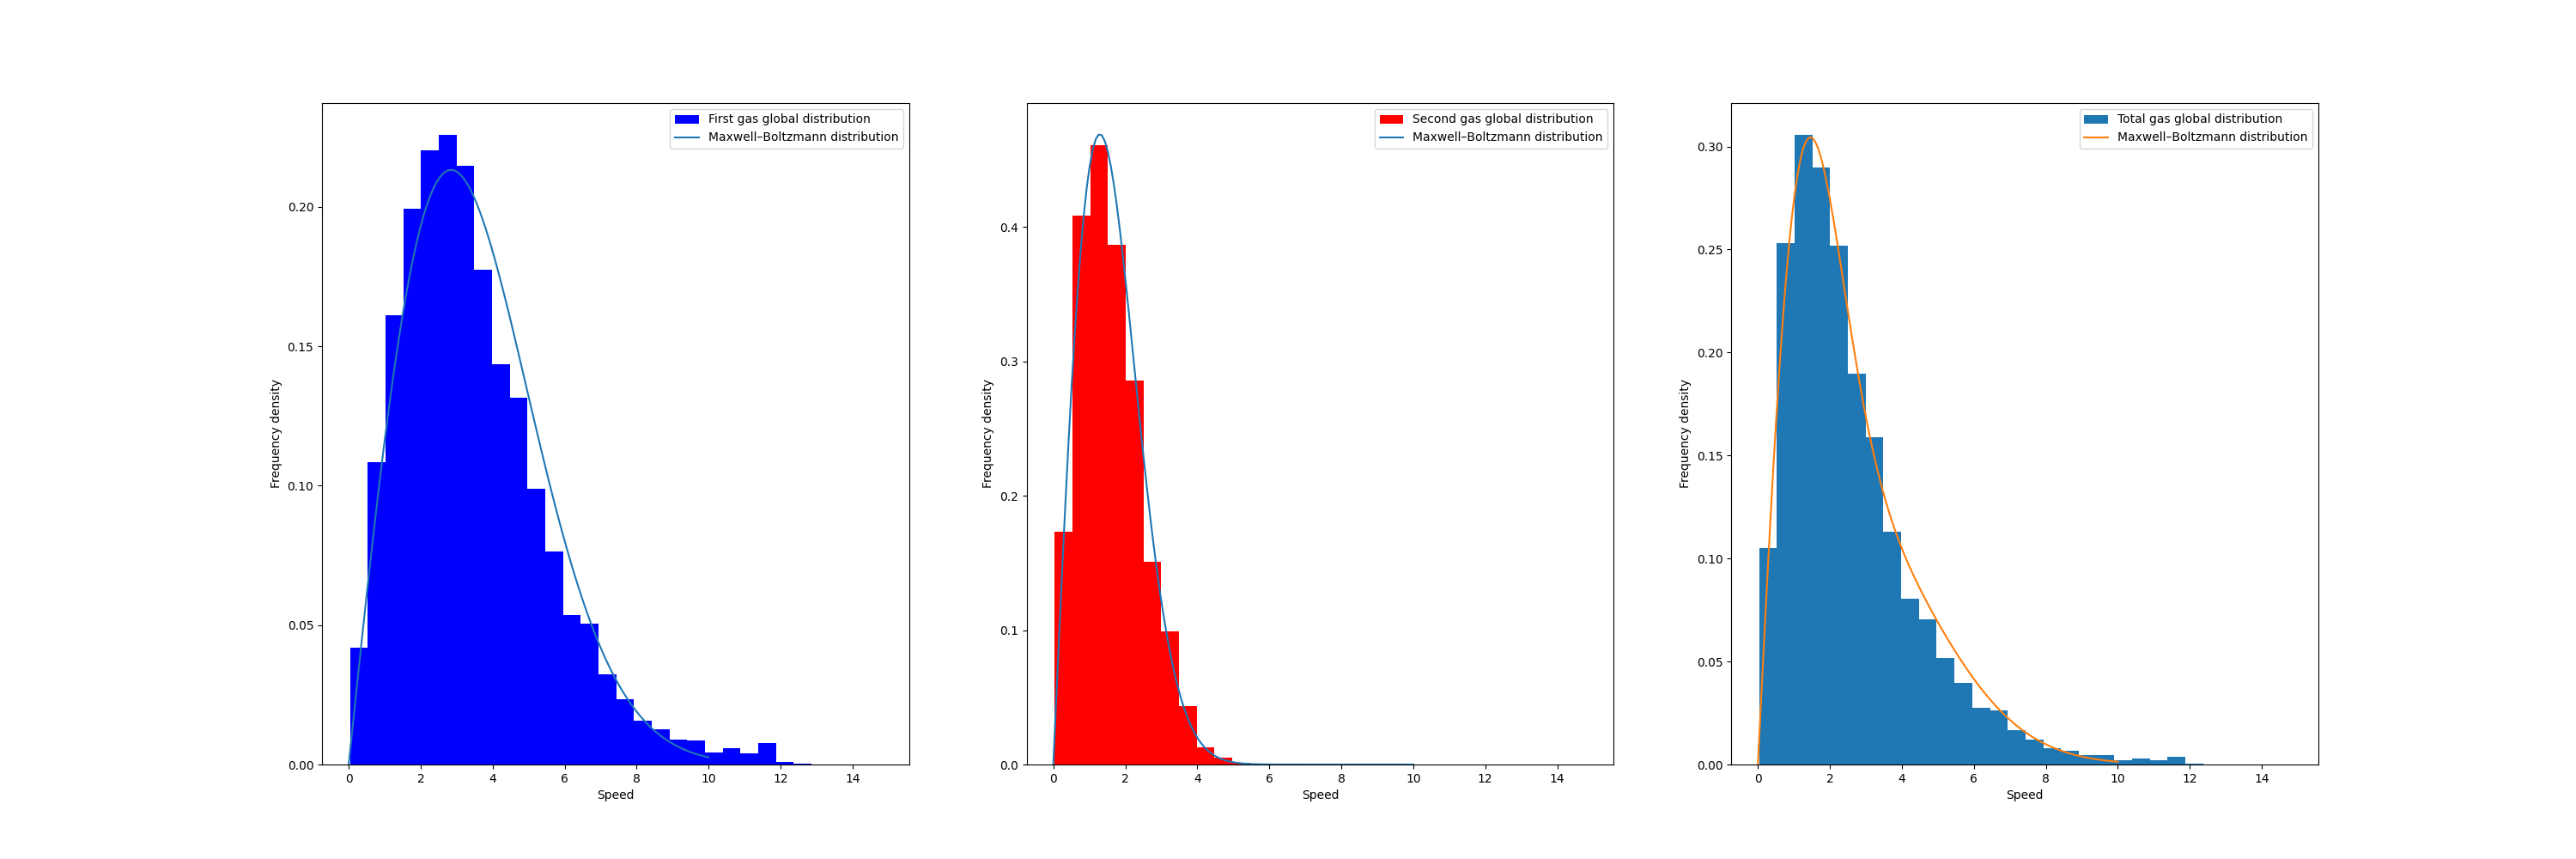
\includegraphics[width=0.8\textwidth]{Mixed_gas_dis.png} % Replace with your image file name
    \caption{Distribution of velocities as explained in the previous section. Each display the distirbution of velocities respectively of the first gas (in blu), the second gas (in red), the combined system of gasses (in light blue) and their theoretical predictions.}
    \label{fig:velocity_distributions} % Label for referencing the figure
\end{figure}

\section{Some more speculations}
\subsection{A new configuration}
In this section, we focus on a specific scenario where collisions occur only with the walls of the box and not between particles. This setup is designed to highlight the significance of inter-particle collisions and their role in leading to the Maxwell-Boltzmann distribution of velocities. By isolating the effects of wall collisions, we aim to clarify how particle interactions contribute to the development of the Maxwell-Boltzmann distribution in a more complex system.
In this scenario, when a particle with a certain velocity magnitude collides with the wall, it is reflected and its direction changes, but its velocity magnitude remains constant (elastic collition). Consequently, if we initialize the particles with a specific velocity magnitude, this magnitude is preserved throughout the simulation. Similarly, if the initial velocity distribution is provided, it remains unchanged throughout the simulation due to the lack of interactions between particles. As a result, the total energy and average energy of the system are conserved, which also implies that the temperature remains constant.

This setup highlights that temperature is not directly tied to the distribution of velocities but rather to the mean value of the velocity distribution. We now pose the question: If all particles are given the same velocity magnitude and their directions are chosen randomly uniformly (assuming isotropy of space), what will be the distribution of the components of the velocities after only wall collisions and no particle-particle collisions? Specifically, will these components follow a Gaussian distribution, or is Gaussianity a feature that emerges from the random collisions between particles?

This investigation aims to clarify whether the Gaussian distribution of velocity components is inherent to the system or a result of interactions between particles.
\subsection{Implementation}

Based on physical assumptions, we can assert that, in the absence of any preferred direction (either \(x\) or \(y\)), the probability density functions (PDFs) of \(v_x\) and \(v_y\) should have the same functional form, though they are functions of different variables. In this setting, each particle maintains a constant velocity magnitude \(v\) throughout the simulation.

To analyze the distributions, we rewrite the velocity components as \(v_x = v \cos(\theta)\) and \(v_y = v \sin(\theta)\), where \(\theta\) is uniformly distributed in the range \([0, 2\pi)\) due to isotropy. Consequently, the PDFs of \(x\) and \(y\) are computed (Check the Appendix section C) and found to be:

\[
f(v_x) = \frac{1}{\pi \sqrt{v^2 - v_x^2}}
\]

\[
f(v_y) = \frac{1}{\pi \sqrt{v^2 - v_y^2}}
\]

As demonstrated, the functional form of \(f(x)\) and \(f(y)\) is identical, and notably, it is not Gaussian. We will verify whether this is indeed the correct PDF by conducting simulations to compare the theoretical and empirical results.


\subsection{Code}
The code used for this simulation is a slightly modified version of the single gas simulation code. Some functions were commented out to adapt the simulation to the current setup. 

In this modified code, we plotted a figure consisting of two histograms. The first histogram shows the distribution of \(v_x\), and the second histogram shows the distribution of \(v_y\). These histograms were created by collecting the velocity components of the particles at the final step of the simulation, after they had collided multiple times with the walls. This allows us to observe how the distribution of velocity components evolves in this particular setup, where collisions are only with the walls and not between particles.

\subsection{Results}
We present the resulting histograms, which show a perfect accordance with the predictions derived in the previous subsections.
% Add a figure with a caption
\begin{figure}[h] % 'h' places the figure approximately here
    \centering
    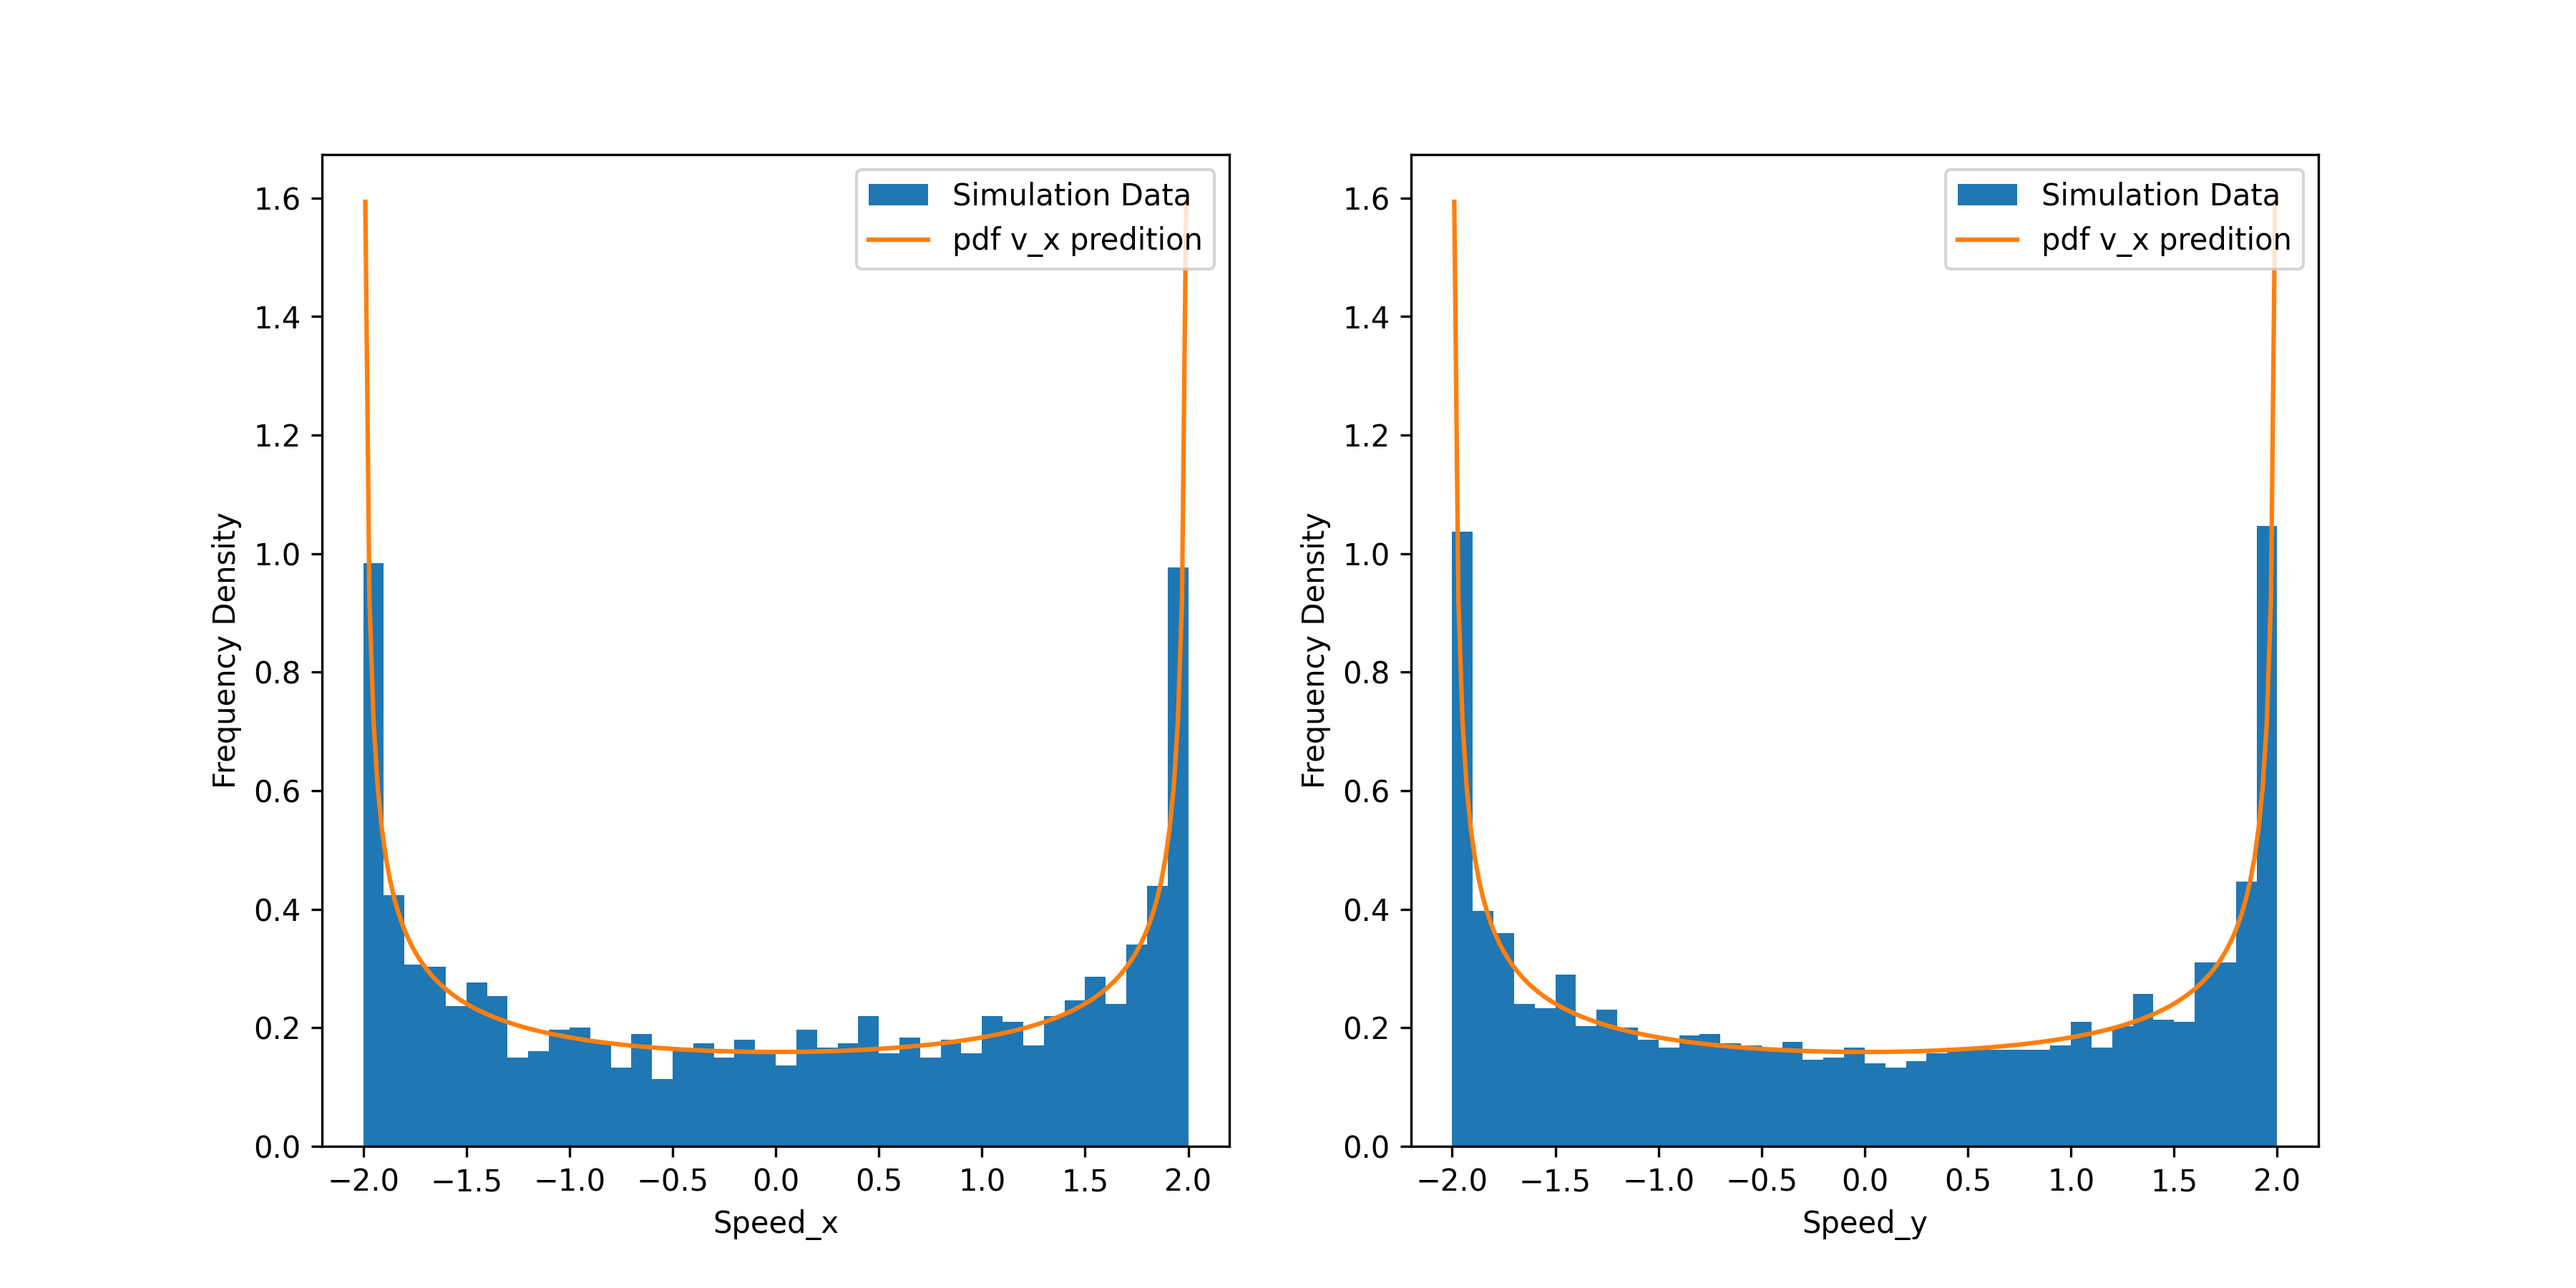
\includegraphics[width=0.8\textwidth]{vel_components.png} % Replace with your image file name
    \caption{Distribution of velocity components as explained in the previous section. In this case the velocity module was set to be equal to 2 u.m.}
    \label{fig:velocity_distribution} % Label for referencing the figure
\end{figure}

The histograms demonstrate that the distributions of \( v_x \) and \( v_y \) are not Gaussian, as predicted by the theoretical analysis in the absence of collisions between particles. This indicates that the Gaussian nature of the velocity component distributions is indeed a result of the random collisions between particles, which was not present in this particular simulation setup.

Thus, we can assert that the Gaussian trait of the velocity component distributions arises from the high number of random collisions between particles, a phenomenon that is evident when particles interact with each other in a typical gas simulation.


% \section{Conclusion}
% The simulation results demonstrate the verification of the Maxwell-Boltzmann distribution and the behavior of gas mixing under different conditions. Future work could involve exploring more complex scenarios and improving simulation accuracy.
\appendix
\section*{Appendix}
\section{Velocity Computation After a Collision}

In this section, we briefly introduce the formulas used to compute the velocities after a collision of two particles. Since we assume the particles have an actual size and are not point-like, and we are considering a two-dimensional impact with conservation of kinetic energy and momentum, the equations for the output velocities after a collision are as follows:

\begin{align}
    \mathbf{v}_1' &= \mathbf{v}_1 - \left( \frac{2m_2}{m_1 + m_2} \right) \left( \frac{\text{scalar\_product}(\mathbf{v}_1 - \mathbf{v}_2, \mathbf{x}_1 - \mathbf{x}_2)}{\|\mathbf{x}_1 - \mathbf{x}_2\|^2} \right) (\mathbf{x}_1 - \mathbf{x}_2) \\
    \mathbf{v}_2' &= \mathbf{v}_2 - \left( \frac{2m_1}{m_1 + m_2} \right) \left( \frac{\text{scalar\_product}(\mathbf{v}_2 - \mathbf{v}_1, \mathbf{x}_2 - \mathbf{x}_1)}{\|\mathbf{x}_2 - \mathbf{x}_1\|^2} \right) (\mathbf{x}_2 - \mathbf{x}_1)
\end{align}

For additional information, refer to \href{https://en.wikipedia.org/wiki/Elastic_collision}{Wikipedia on Elastic Collisions}.

One brief notice: Let us highlight the non-guaranteed fact that, in the case of particles with the same masses and non-zero size, which have the same velocity magnitude before the impact, they might not have the same velocity magnitude after the collision.


\section{Generalization to $n$ Gases and Calculation of Equilibrium Temperature}
\label{sec:appendix}

In this section of the appendix, we generalize the discussion to the mixing of \(n\) gases. This extension is a straightforward application of Bayes' theorem, as was done in the simplified case with two gases in the previously cited section.

Thus, we can express the cumulative probability density function (PDF) for the velocity magnitude \(v\) as:

\[
f_{\text{cumulative}}(v) = \sum_{i=1}^{n} f_i(v) P_i
\]

where \(f_i(v)\) is the PDF of the \(i\)-th gas, and \(P_i = \frac{N_i}{N_{\text{total}}}\). Here, \(N_i\) is the number of particles in the \(i\)-th gas, and \(N_{\text{total}} = \sum_{i=1}^{n} N_i\) is the total number of particles.

Since we know that the individual PDFs \(f_i(v)\) are Rayleigh distributions, we can write:

\[
f_{\text{cumulative}}(v) = \sum_{i=1}^{n} \left( \frac{v}{\sigma_i^2} \right) \exp\left(-\frac{v^2}{2\sigma_i^2}\right) P_i
\]

where \(\sigma_i = \sqrt{\frac{k_B T_i}{m_i}}\), with \(T_i\) and \(m_i\) being the temperature and mass of the \(i\)-th gas, respectively, and \(k_B\) is the Boltzmann constant.

By substituting this expression and factoring out the non-indexed quantities, we obtain:

\[
f_{\text{cumulative}}(v) = \left( \frac{v}{k} \right) \exp\left(-\frac{v^2}{2k}\right) \sum_{i=1}^{n} \left( \frac{m_i}{T_i} \right) \exp\left(-\frac{m_i}{T_i}\right) P_i
\]

In the special case where the gases are thermalized (all at the same temperature \(T\)), we can factor out \(T\) and rewrite the expression as:

\[
f_{\text{cumulative}}(v) = \left( \frac{v}{kT} \right) \exp\left(-\frac{v^2}{2kT}\right) \sum_{i=1}^{n} m_i \exp\left(-m_i\right) \frac{N_i}{N_{\text{total}}}
\]

If desired, we can substitute \(N_i\) and \(N_{\text{total}}\) using the ideal gas relation:

\[
N_i = \frac{P_i V N_A}{R T}, \quad N_{\text{total}} = \frac{P V N_A}{R T}
\]

where \(P_i\) and \(P\) are the partial pressures of the \(i\)-th gas and the total pressure, respectively, and \(N_A\) is Avogadro's number. Simplifying this, we leave the equation as a function of the partial pressures.


\section{Calculating \(v_x\) and \(v_y\) PDF from Uniformly Distributed \(\theta\)}
\label{sec:appendix}

In this section, we expand on the calculations that allow us to determine the distributions of \(v_x\) and \(v_y\), assuming the gas molecules have a constant velocity (colliding only with walls) and the same speed \(v\), exploiting the relations \(v_x = v \cos \theta\) and \(v_y = v \sin \theta\), where \(\theta\) is uniformly distributed between 0 and \(2\pi\) (isotropy).

We begin by defining the cumulative distribution function (CDF) for \(v_x\):

\[
P(v_x < V_x) = P(v \cos \theta < V_x)
\]

Solving the inequality \(v \cos \theta < V_x\) in the range \(0\) to \(2\pi\), we obtain:

\[
P\left(\arccos\left(\frac{V_x}{v}\right) < \theta < 2\pi - \arccos\left(\frac{V_x}{v}\right)\right)
\]

By the definition of the cumulative distribution function \(F_\theta\), this becomes:

\[
F_\theta(2\pi - \arccos(V_x/v)) - F_\theta(\arccos(V_x/v))
\]

Taking the derivative of this expression with respect to \(V_x\), we obtain the probability density function (PDF) of \(v_x\):

\[
f_{v_x}(V_x) = f_\theta(2\pi - \arccos(V_x/v)) \left(\frac{-1}{v \sqrt{1 - \frac{V_x^2}{v^2}}}\right) - f_\theta(\arccos(V_x/v)) \left(\frac{1}{v \sqrt{1 - \frac{V_x^2}{v^2}}}\right)
\]

Since \(f_\theta = \frac{1}{2\pi}\), we simplify the equation to:

\[
f_{v_x}(V_x) = \frac{1}{v 2\pi} \frac{1}{\sqrt{v^2 - V_x^2}} + \frac{1}{v 2\pi} \frac{1}{\sqrt{v^2 - V_x^2}}
\]

Thus, we obtain the PDF:

\[
f_{v_x}(V_x) = \frac{1}{\pi \sqrt{v^2 - V_x^2}}
\]

A similar calculation can be performed to find the PDF of \(v_y\). Therefore, we observe that the shape of these two PDFs is the same, as expected from physical intuition.


We would like to further test this function and show that it fulfills another condition, which is derived assuming the PDFs of \(v_y\) and \(v_x\) muust be the same. 
A first approach that we used to find the correct PDF of the velocities was the following:

We know that \(v_x\) and \(v_y\) are linked by the relation \(v_x^2 + v_y^2 = v^2\), and due to the fact that in this case \(v\) is constant (no interaction between particles), the distributions of \(v_x\) and \(v_y\) are not independent.

Therefore, we wanted to use the following trick:
Let us suppose we know the PDF of \(v_x\) and try to derive the PDF of \(v_y\).

We know that \(v_y = \pm \sqrt{v^2 - v_x^2}\).

We start by studying the distribution of \(v_y = + \sqrt{v^2 - v_x^2}\), which implicitly leads us to study the PDF of \(\vert v_y \vert\).

We write:

\[
P(\vert v_y \vert < V_y) = P(\sqrt{v^2 - v_x^2} < V_y)
\]

We first notice that if \(V_y < 0\), the probability is null since the square root returns positive values. We therefore study the case where \(V_y > 0\).

By solving the inequality \(\sqrt{v^2 - v_x^2} < V_y\), we get \(v_x < - \sqrt{v^2 - V_y^2}\) or \(\sqrt{v^2 - V_y^2} < v_x\).

Thus, the previous equality with probabilities becomes:

\[
P(v_x < -\sqrt{v^2 - V_y^2} \text{ or } \sqrt{v^2 - V_y^2} < v_x)
\]

By the definition of the cumulative distribution function of \(v_x\), we can rewrite this as:

\[
F_{v_x}(-\sqrt{v^2 - V_y^2}) + 1 - F_{v_x}(\sqrt{v^2 - V_y^2})
\]

By deriving and rearranging some terms, we obtain the PDF of \(\vert v_y \vert\):

\[
f_{\vert v_y \vert}(v_y) = \frac{v_y}{\sqrt{v^2 - V_y^2}} \left( f_{v_x}(\sqrt{v^2 - V_y^2}) + f_{v_x}(-\sqrt{v^2 - V_y^2}) \right)
\]

We now suppose that, for symmetry reasons, \(f_{v_x}\) (and then \(f_{v_y}\)) is an even function, and thus:

\[
f_{\vert v_y \vert}(v_y) = \frac{2v_y}{\sqrt{v^2 - V_y^2}} f_{v_x}(\sqrt{v^2 - V_y^2})
\]

As we mentioned before, we impose that \(f_{\vert v_y \vert}(v_y) = f_{\vert v_x \vert}(v_x)\), and this needs to be equal to \(2f_{v_x}(v_y)\) because we want both distributions to have the same shape.

Therefore, the correct \(f_{v_x}\) (and \(f_{v_y}\)) needs to satisfy the relation:

\[
\frac{2v_y}{\sqrt{v^2 - V_y^2}} f_{v_x}(\sqrt{v^2 - V_y^2}) = 2 f_{v_x}(v_y)
\]

It's easy to show that the \(f_{v_x}\) found earlier satisfies this equation.

One might argue that there are several other functions that respect this condition, such as \(f_{v_x} = C \vert v_x \vert\) or equivalently \(f_{v_y} = C \vert v_y \vert\).

Therefore, one might ask what makes the PDF found above a better solution than this second one?

It is because the PDF we derived is linked to the uniformly distributed \(\theta\), in accordance with the isotropy of space, whereas the alternative functions are not associated with \(\theta\) being uniformly distributed (i.e., some directions would be privileged).



% \begin{thebibliography}{9}

% \bibitem{reference1}
% Author Name,
% \textit{Title of the Book or Paper},
% Publisher, Year.

% \end{thebibliography}

\end{document}
